\documentclass{experimentreport}

\usepackage{graphicx}

\input{listing_style.tex}

%========================
% Basic Information
%========================

\setcoursename{Practical Training in Basic Software Development Technologies}
\setreportname{Intelligent Software Engineering Experiment Report}

\setexperimenttitle{\hintholder{Please enter the experiment title}}

\setstudentname{\hintholder{Please enter your name}}
\setdepartment{\hintholder{Please enter your department}}
\setstudentid{\hintholder{Please enter your student ID}}

\setcourseteacher{Liu Jiakun}
\setinstructor{Liu Jiakun}

\setlablocation{\hintholder{Please enter the lab location}}
\setlabtime{\hintholder{Please enter the lab time}}

\begin{document}

\graphicspath{{./}}

%========================
% Automatically Generate Cover Page
%========================

\makereporthead

%========================
% Experiment Objectives
%========================

\experimentpurpose{

- Understood PR and code review workflows in modern development.
- Learned GitHub repository code review data structure.
- Mastered relationships between PRs, commits, reviews, and comments.
- Retrieved code review data via GitHub API.
- Extracted code, text, and metadata from PRs.
- Applied statistical analysis to build dataset for subsequent experiments.

}

%========================
% Experiment Content
%========================

\experimentcontent{
- Selected 5 projects: pytorch, tensorflow, kubernetes, vscode, langchain.
- Retrieved 300 PRs per project (1,550 total after trimming).
- Extracted PR metadata: ID, title, body, author, creation time, merge status.
- Retrieved reviews: reviewer, decision, time, comment text.
- Extracted commits: messages and diff content.
- Collected labels from each PR.
- Detected AI reviewers using keyword matching.
- Detected AI-generated code using keyword matching.
- Performed statistical analysis on the full dataset.
}

%========================
% Experiment Results
%========================

\experimentresult{
We collected 1,550 PRs from 5 open-source projects. Key statistics:
- 813 merged (52.5\%), 737 unmerged (47.5\%).
- Average additions: 9,110 lines.
- Average deletions: 428 lines.
- Average changed files: 88.
- Average reviewers per PR: 1.8.
- Average review comments per PR: 1.6.
- AI reviewers present in 471 PRs (30.4\%).
- AI-generated code detected in 530 PRs (34.2\%).

Six visualizations were produced showing merge status, review comments distribution, reviewers per PR, PR length, AI vs human code comparison, and top 10 labels.

\begin{figure}[h]
\centering
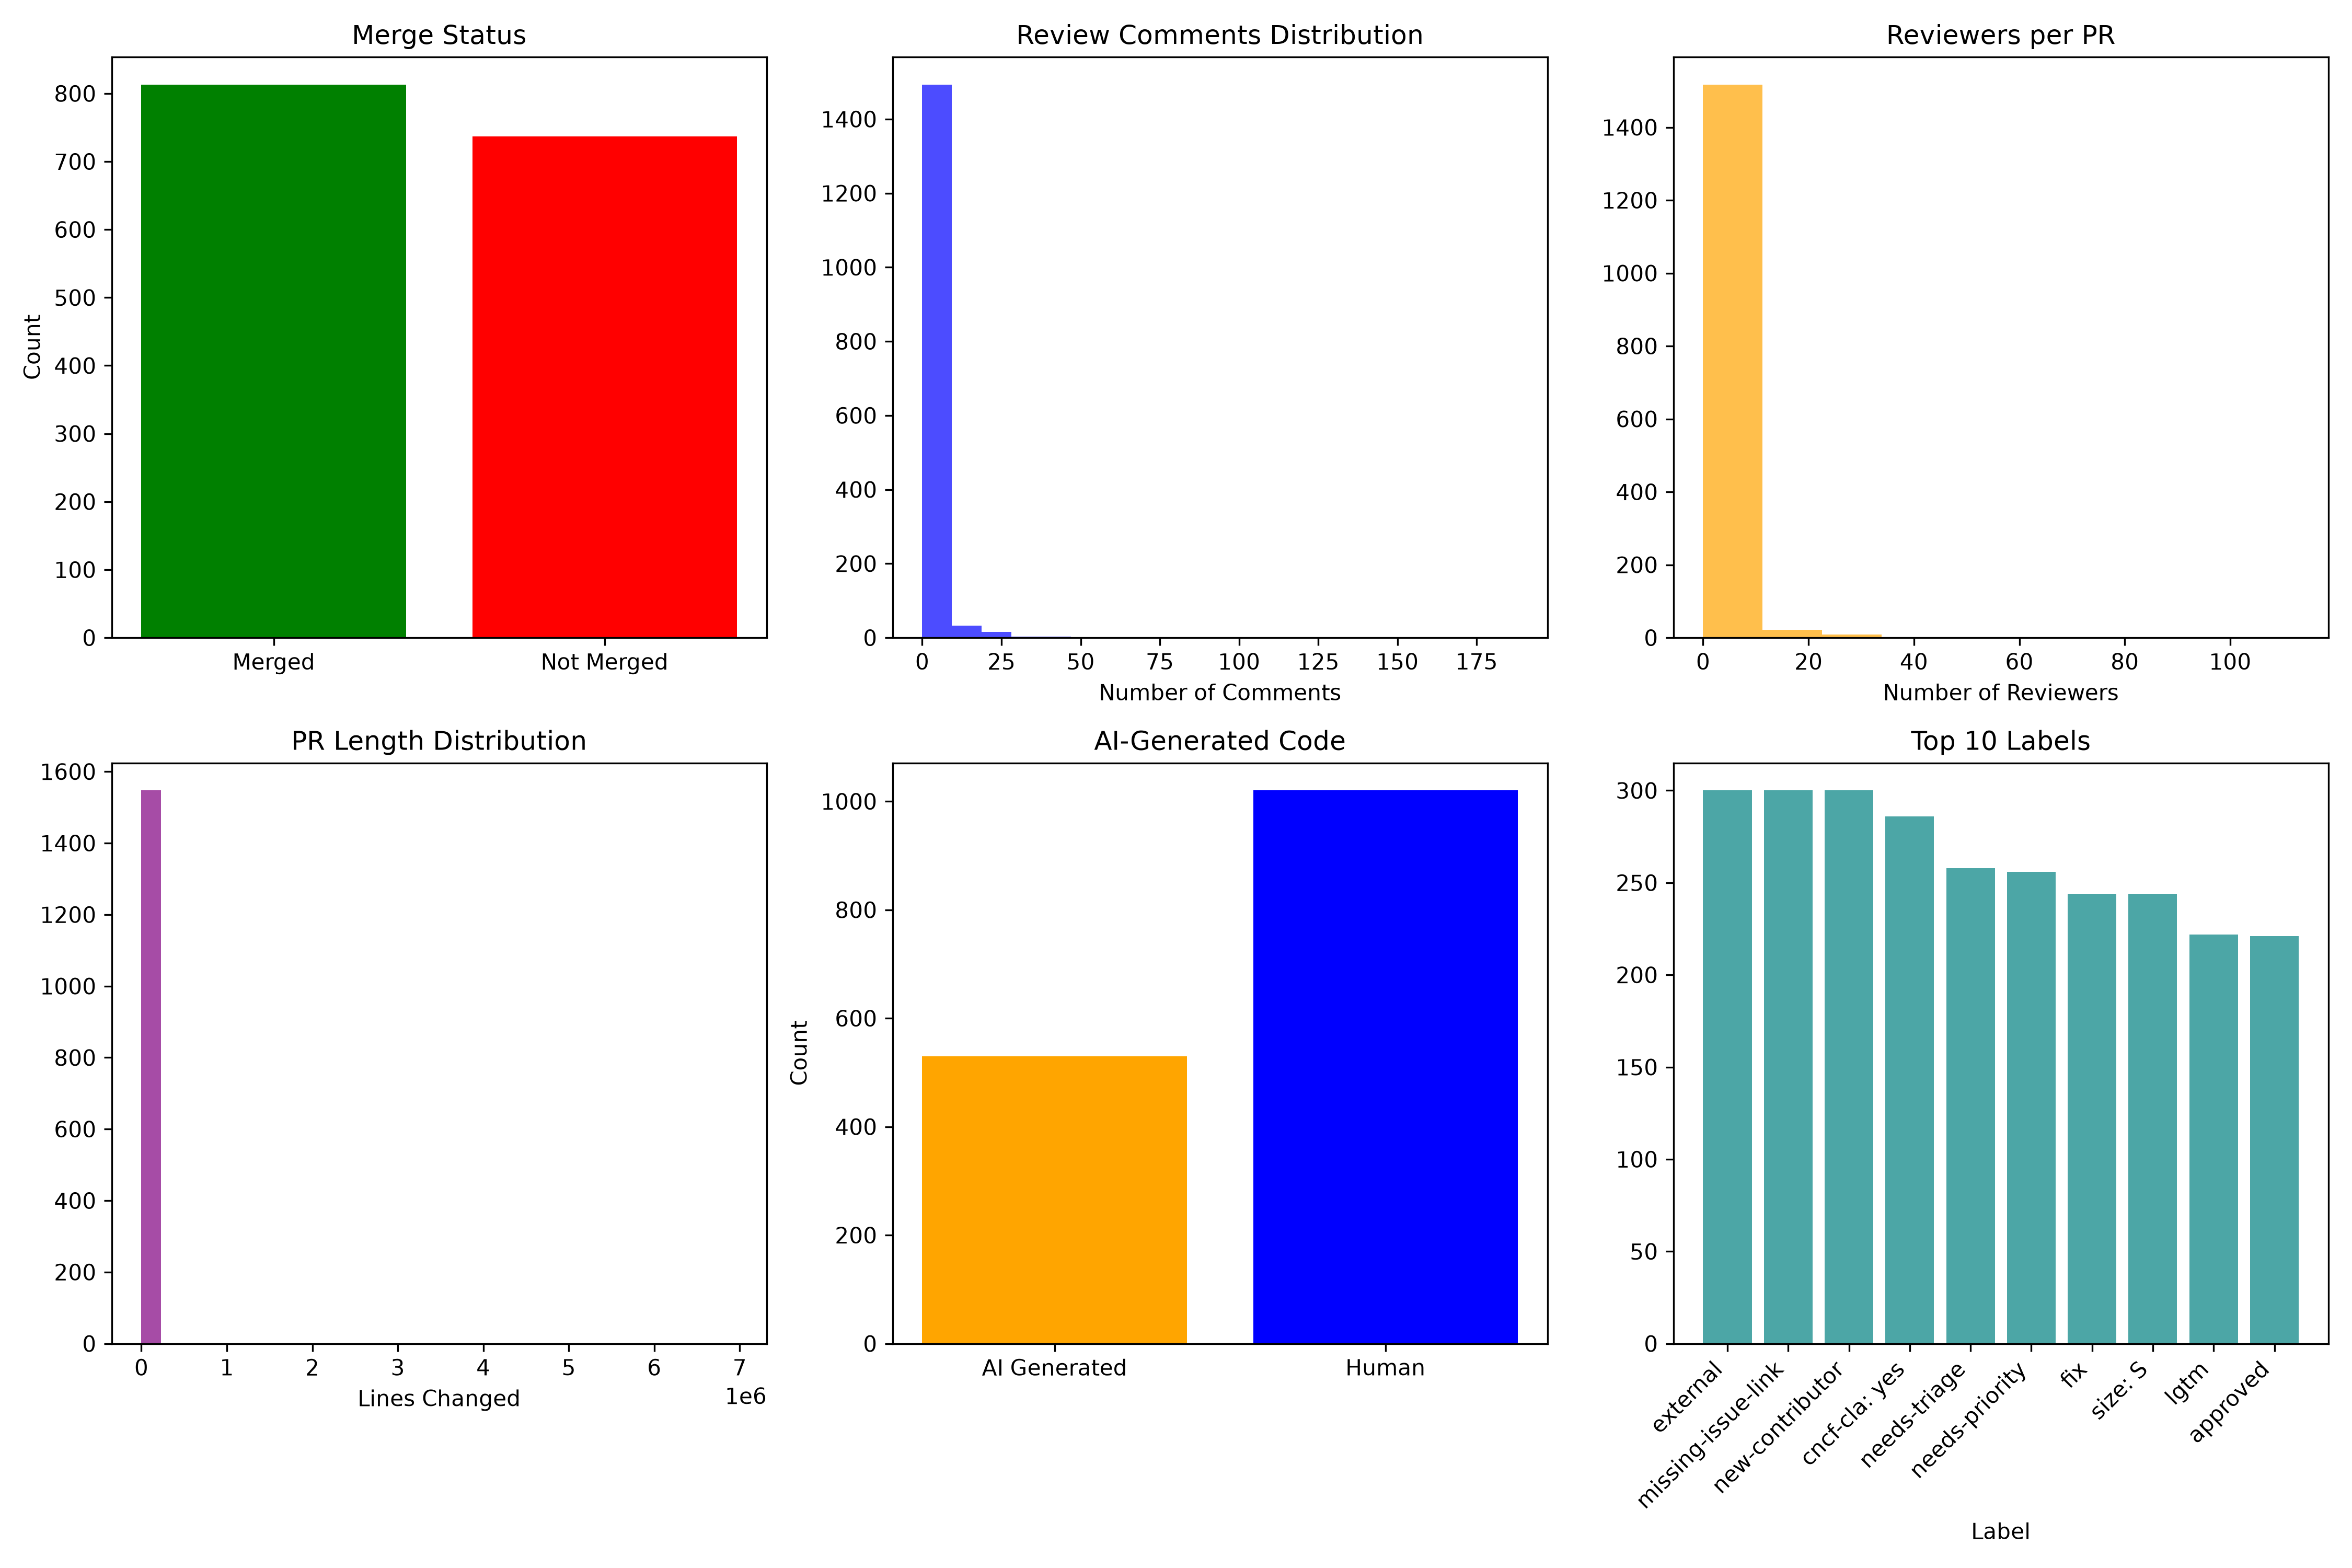
\includegraphics[width=\textwidth]{analysis_plots.png}
\caption{Statistical analysis of the PR dataset}
\end{figure}
}

%========================
% Summary of Issues
%========================

\experimentproblems{
- API rate limiting: added 0.15s delays between requests.
- Network interruptions: implemented checkpoint saving every 5 PRs.
- Langchain contained 9,450 PRs. Trimmed to 300 most recent for balanced distribution.
- PyGithub deprecation warnings. Code functions correctly despite warnings.
}

%========================
% Reflections
%========================

\experimentexperience{
- PR is a merge request containing discussion and multiple commits. A commit is a single code change.
- Code review catches defects early, enforces standards, and spreads knowledge across the team.
- Merge prediction can flag high-risk PRs, prioritize reviews, and automate CI decisions.
- AI reviewers respond instantly but lack project-specific context. Human reviewers understand broader design implications.
- Our dataset has moderate imbalance (52.5\% merged). SMOTE or class weighting can address this.
}

%========================
% Instructor Comments
%========================

\teachercomment

\end{document}